\documentclass{article}
\usepackage[utf8]{inputenc}
\usepackage[a4paper, total={6in, 10in}]{geometry}

\title{Treinamento Matrix}
\author{Yudi Yamane}
\date{Fevereiro 2020}

\usepackage{listings}
\usepackage{parskip}
\usepackage{natbib}
\usepackage{hyperref}
\usepackage{graphicx}
\hypersetup{
    colorlinks=true,
    linkcolor=cyan,
    filecolor=magenta,  
    urlcolor=blue,
}


\begin{document}

\maketitle

\section{Introdução}
Nesse treinamento vamos aprender algumas ferramentas básicas de web pra imitar a chuva de código 
do filme Matrix. O resultado pode ser visualizado \href{https://yudi-azvd.github.io/matrix/}{aqui}. 
E esse trabalho foi inspirado pelo \href{https://www.youtube.com/watch?v=S1TQCi9axzg}{tutorial} da Emily Xie.

Para desenvolver esse projeto vamos utilizar HTML, CSS e JavaScript. Esse projeto poderia ser
desenvolvido em C, Java ou Python, usando bibliotecas de animação ou não. Entretanto, o objetivo
principal desse treinamento é aprender alguns conceitos e técnicas de programação pra melhorar a 
qualidade e legibilidade de código. Conceitos e técnicas como \textbf{abstração}, 
\textbf{divisão de problemas em subproblemas}, e \textbf{convenções} para nomeação de variáveis 
e entre outros.

Antes de prosseguir certifique-se de ter algum editor de texto voltado para programação 
instalado em seu computador. Recomendo fortemente o 
\href{https://code.visualstudio.com/}{Visual Studio Code}(VS code). Outros como 
\href{https://www.sublimetext.com/}{Sublime Text} ou 
\href{https://atom.io/}{Atom} também são muito bons.

\section{Ferramentas}
\subsection{HTML}
\subsubsection{Geral}
Significa \textit{HyperText Markup Language} e define a \textbf{estrutura} e \textbf{significado} 
dos elementos de página web. Usando um prédio como comparação, o HTML seria as vigas, o cimento, 
os buracos para as janelas, os espaços para os encanamentos e fiação elétrica e etc.

Hypertext se refere ao fato de muitas dessas páginas estarem ligadas umas as outras através de links,
criando assim uma grande rede que compõe parte da World Wide Web.

Markup se refere ao fato de o texto HTML ser marcado por "tags" que definem os elementos usados 
na página. Vamos dar uma olhada em como isso ficaria em código:

\begin{figure}[h!]
    \centering
    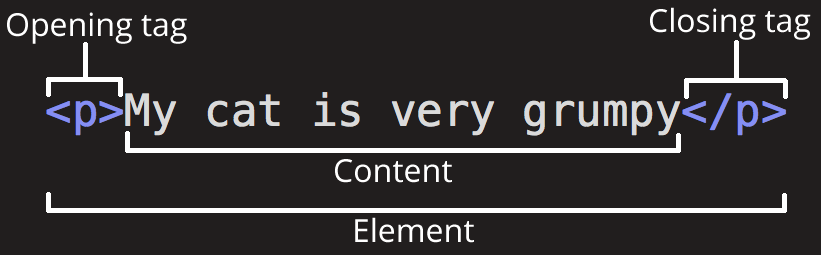
\includegraphics[scale=.4]{imgs/element-anatomy.png}
    \caption{Anatomia geral de um elemento HTML.}
    \label{fig:element-anatomy}
\end{figure}


\begin{itemize}
\item
  \textbf{tag de abertura:} é o nome do elemento envolvido por
  \texttt{\textless{}} à esquerda e por \texttt{\textgreater{}} à
  direita.
\item
  \textbf{tag de fechamento:} é o nome do elemento envolvido por
  \texttt{\textless{}/} à esquerda e por \texttt{\textgreater{}} à
  direita Note a presença da barra normal. Além disso, é válido
  mencionar que nem todos os elementos precisam de uma tag de
  fechamento. De maneira de geral quando ela não tem um conteúdo a tag
  de fechamento pode ser desconsiderada.
\item
  \textbf{conteúdo:} é o que vai entre as tags. Pode ser texto como na
  imagem ou até mesmo outros elementos como veremos mais pra frente.
\item
  \textbf{elemento =} tag de abertura \textbf{+} conteúdo \textbf{+} tag
  de fechamento (novamente, de maneira geral)
\end{itemize}

Para conhecer outros elementos, clique
\href{https://developer.mozilla.org/en-US/docs/Web/HTML/Element}{aqui}.


\subsubsection{Atributos}
Além disso, elementos HTML podem possuir atributos:

\begin{figure}[h!]
    \centering
    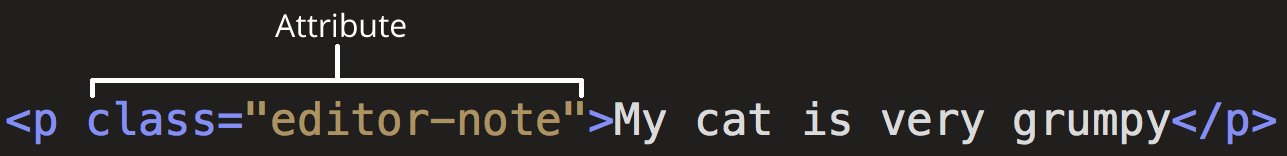
\includegraphics[scale=.3]{imgs/attrs.png}
    \caption{Anatomia geral de um elemento HTML.}
    \label{fig:attrs}
\end{figure}

Atributos são informações adicionais que passamos para os elementos.
Eles não aparecem no conteúdo. No caso da imagem, o atributo
\texttt{class} dá uma característica especial para esse elemento.
Veremos mais sobre \texttt{class} mais pra frente.


Vamos usar um editor de texto agora pra visualizar essas coisas. Crie
uma pasta chamada \texttt{matrix} no seu computador em um lugar que seja
conveniente pra você e abra essa pasta no seu editor. Para fazer isso,
geralmente é \emph{File} \textgreater{} \emph{Open Folder.}

Crie um arquivo \texttt{index.html} e abra-o no editor. Escreva o
seguinte:

%%% FOTO DO CÓDIGO HTML DE CORPO INTEIRO

No elemento \texttt{a} (link), \texttt{href} é outro tipo atributo que
indica ou ``vai'' para outra página ou recurso na internet.


\subsubsection{Visualização do HTML}
Podemos visualizar o resultado do que escrevemos de pelo menos duas
formas:

\begin{enumerate}
\item
  Abra o navegador de sua preferência (Chrome, Firefox, Edge) e arraste
  o arquivo \texttt{index.html} para o navegador. Se utilizarmos essa
  forma, temos que atualizar (\emph{a cada} alteração) a página do
  navegador para visualizarmos as alterações que fizermos no código.
\item
  Outra forma é utilizando uma extensão que existe para editores de
  texto. Essa extensão abre um servidor no nosso computador que escuta
  por alterações nos arquivos e atualiza a página automaticamente caso
  aconteçam.
\end{enumerate}

Para instalar o plugin no VSCode use o atalho \texttt{Ctrl+shift+x} (ou
clique no último ícone da barra lateral esquerda) para abrir a loja de
extensões e procure por Live Server e clique nela. Clique em ``Install''.
Você deve ver algo parecido com a Figura \ref{fig:live-server-ext}.

\begin{figure}[h!]
    \centering
    
\includegraphics[scale=.5]{imgs/live-server-extension.png}
    \caption{Foto da extensão.}
    \label{fig:live-server-ext}
\end{figure}

A loja de extensões no VS code é muito rica. Extensões servem para
ajudar o programador a programar seja corrigindo um trecho de código
automaticamente seja incorporando uma série de atalhos para geração
automática de código para algumas linguagens (para mais sugestões clique
nesse
\href{https://www.ubuntupit.com/best-visual-studio-code-extensions-for-programmers/}{link}).
Além dessas úteis, existem também algumas de zoerinha como a extensão
\href{https://marketplace.visualstudio.com/items?itemName=hoovercj.vscode-power-mode}{Power
Mode}.

\begin{figure}[h!]
    \centering
    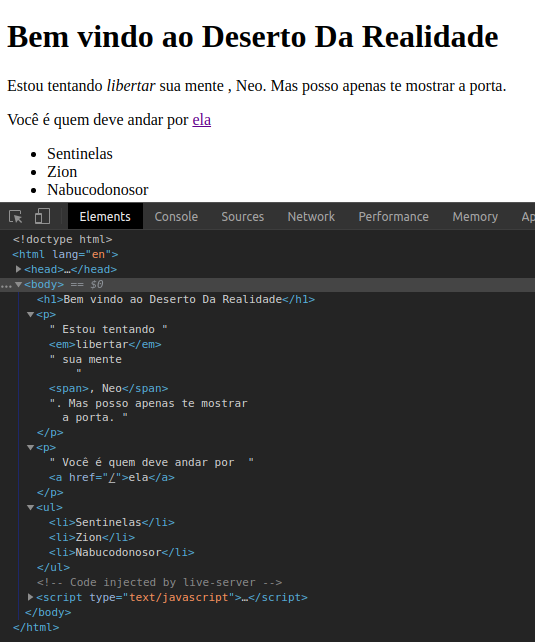
\includegraphics[scale=.5]{imgs/page-chr-dev-tools.png}
    \caption{HTML renderizado na página com o painel DevTools do Chrome aberto.}
    \label{fig:page-chr-dev-tools}
\end{figure}

\newpage
\section{Conclusion}
``I always thought something was fundamentally wrong with the universe'' \citep{adams1995hitchhiker}

lorem ipsumlorem ipsum ipsumlorem ipsum i
psumlorem ipsum ipsumlorem ipsum ipsumlorem ipsum ip
sumlorem ipsum ipsumlorem ipsum ipsumlorem ipsum ipsumlore
m ipsum ipsumlorem ipsum ipsumlorem ipsum ipsumlorem ipsum ipsumlorem ipsum ipsuml
orem ipsum ipsumlorem ipsum 
ipsumlorem ipsum ipsumlorem ipsum 


\bibliographystyle{plain}
\bibliography{references}
\end{document}
